% Created 2011-10-19 Wed 22:55
\documentclass[bigger]{beamer}
\usepackage[utf8]{inputenc}
\usepackage[T1]{fontenc}
\usepackage{fixltx2e}
\usepackage{graphicx}
\usepackage{longtable}
\usepackage{float}
\usepackage{wrapfig}
\usepackage{soul}
\usepackage{textcomp}
\usepackage{marvosym}
\usepackage{wasysym}
\usepackage{latexsym}
\usepackage{amssymb}
\usepackage{hyperref}
\tolerance=1000
\usetheme[titlepagelogo=lal-logo]{Binet}
\usepackage{minted}
\usemintedstyle{emacs}
\pgfdeclareimage[height=1.5cm]{lal-logo}{lal-logo-eps-converted-to}
\logo{\pgfuseimage{lal-logo}}
\hypersetup{colorlinks,linkcolor=blue,urlcolor=blue}
\providecommand{\alert}[1]{\textbf{#1}}

\title{Musings with `Go' - addressing the multicore issues of today and the manycore problems of tomorrow ?}
\author{S\'ebastien Binet}
\date{2011-10-20}

\institute[LAL]{\insertlogo\hskip0.1cm}
\begin{document}

\maketitle





\section{go in HEP}
\label{sec-1}
\begin{frame}
\frametitle{Introduction}
\label{sec-1-1}


\begin{itemize}
\item Moore's law ceased to provide the traditional single-threaded
  performance increases
\begin{itemize}
\item clock-frequency wall of 2003
\item still deliver increases in \alert{transistor density}
\end{itemize}
\item multicore systems become the norm
\item need to ``go parallel'' to get scalability
\end{itemize}
\end{frame}
\begin{frame}
\frametitle{In a \verb~C++~ world\ldots{}}
\label{sec-1-2}

\begin{itemize}
\item parallel programming in \verb~C++~ is \alert{doable}:
\begin{itemize}
\item \verb~C/C++~ ``locking + threads'' (\verb~pthreads~, \verb~WinThreads~)
\begin{itemize}
\item excellent performance
\item good generality
\item relatively \alert{low productivity}
\end{itemize}
\item multi-threaded applications\ldots{}
\begin{itemize}
\item hard to get right
\item hard to \alert{keep} right
\item hard to \alert{keep} efficient and optimized across releases
\end{itemize}
\item multi-process applications\ldots{}
\begin{itemize}
\item \`a la \verb~AthenaMP/GaudiMP~
\item leverage \verb~fork+COW~ on \verb~GNU/Linux~
\item event-level based parallelism
\end{itemize}
\end{itemize}
\end{itemize}
\begin{block}{\quad}
\label{sec-1-2-1}

 \begin{center}
 Parallel programming in ~C++~ is \alert{doable}, \\
 but \alert{\emph{no panacea}}
 \end{center}
\end{block}
\end{frame}
\begin{frame}
\frametitle{In a \verb~C++~ world\ldots{}}
\label{sec-1-3}

\begin{itemize}
\item in \verb~C++03~, we have libraries to help with parallel programming
\begin{itemize}
\item \verb~boost::lambda~
\item \verb~boost::MPL~
\item \verb~boost::thread~
\item Threading/Array Building Blocks (TBB/ArBB)
\item Concurrent Collections (CnC)
\item \verb~OpenMP~
\item \ldots{}
\end{itemize}
\end{itemize}
\end{frame}
\begin{frame}
\frametitle{In a \verb~C++11~ world\ldots{}}
\label{sec-1-4}

\begin{itemize}
\item in \verb~C++11~, we get:
\begin{itemize}
\item $\lambda$ functions (and a new syntax to define them)
\item \verb~std::thread~,
\item \verb~std::future~,
\item \verb~std::promise~
\end{itemize}
\end{itemize}
\begin{block}{\quad}
\label{sec-1-4-1}

 \begin{center}
 Helps taming the beast \\
 ... at the price of sprinkling templates everywhere... \\
 ... and complicating further a not so simple language...
 \end{center}
\end{block}
\end{frame}
\begin{frame}
\frametitle{In a \verb~C++11~ world\ldots{}}
\label{sec-1-5}
\begin{block}{\quad}
\label{sec-1-5-1}

yay! for \verb~C++11~, but old problems are \alert{still there\ldots{}}
\end{block}
\quad
\label{sec-1-5-2}


\begin{itemize}
\item \alert{build scalability}
\begin{itemize}
\item templates
\item headers system
\item still no module system (WG21 - N2073)
\begin{itemize}
\item maybe in the next Technical Report ?
\end{itemize}
\end{itemize}
\end{itemize}

\vspace

\begin{itemize}
\item \alert{code distribution}
\begin{itemize}
\item no \verb~CPAN~ like readily available infrastructure (and cross-platform) for \verb~C++~
\item remember \verb~ROOT/BOOT~ ? (CHEP-06)
\end{itemize}
\end{itemize}
 
\end{frame}
\begin{frame}
\frametitle{Time for a new language ?}
\label{sec-1-6}
\begin{quotation} % \quad
\label{sec-1-6-1}

 ``Successful new languages build on existing languages and where possible, support legacy software. C++ grew our of C. java grew out of C++. To the programmer, they are all one continuous family of C languages.''
 (T. Mattson)
\end{quotation}
\quad
\label{sec-1-6-2}


\begin{itemize}
\item notable exception (which confirms the rule): \alert{python}
\end{itemize}
\begin{alertblock}{\quad}
\label{sec-1-6-3}

    Can we have a language:
\begin{itemize}
\item as easy as \alert{python},
\item as fast (or nearly as fast) as \verb~C/C++/FORTRAN~,
\item with none of the deficiencies of \verb~C++~,
\item and is multicore/manycore friendly ?
\end{itemize}
\end{alertblock}
\end{frame}
\begin{frame}
\frametitle{\quad}
\label{sec-1-7}


\begin{center}
Why not {\texttt Go} ?\\
\href{http://golang.org}{{\color{blue}golang.org}}
\end{center}
\end{frame}
\begin{frame}[fragile]
\frametitle{Elements of \verb~go~}
\label{sec-1-8}


\begin{itemize}
\item obligatory \verb~hello world~ example\ldots{}
\end{itemize}


\begin{minted}[]{go}
package main
import "fmt"
func main() {
    fmt.Println("Hello, World")
}
\end{minted}





\includegraphics[width=.9\linewidth]{figs/golang-logo.pdf}
\end{frame}
\begin{frame}
\frametitle{Elements of \verb~go~ - II}
\label{sec-1-9}


\begin{itemize}
\item founding fathers:
\begin{itemize}
\item Russ Cox, Robert Griesemer, Ian Lance Taylor
\item Rob Pike, Ken Thompson
\end{itemize}
\item concurrent, compiled
\item \alert{garbage collected}
\item an open-source general programming language
\item best of both `worlds':
\begin{itemize}
\item feel of a \alert{dynamic language}
\begin{itemize}
\item limited verbosity thanks to \textbf{type inference system}, map, slices
\end{itemize}
\item safety of a \alert{static type system}
\item compiled down to machine language (so it is fast)
\begin{itemize}
\item goal is within 10\% of \alert{C}
\end{itemize}
\end{itemize}
\item \alert{object-oriented} (but w/o classes), \alert{builtin reflection}
\item first-class functions with \alert{closures}
\item \alert{duck-typing} \`a la \verb~python~
\end{itemize}
\end{frame}
\begin{frame}
\frametitle{\verb~Go~ concurrent}
\label{sec-1-10}
\begin{block}{goroutines}
\label{sec-1-10-1}


\begin{itemize}
\item a function executing concurrently as other goroutines \alert{in the same address space}
\item starting a goroutine is done with the \verb~go~ keyword
\begin{itemize}
\item \verb~go myfct(arg1, arg2)~
\end{itemize}
\item growable stack
\begin{itemize}
\item \alert{lightweight threads}
\item starts with a few kB, grows (and shrinks) as needed
\begin{itemize}
\item now, also available in \verb~GCC~ 4.6 (thanks to the \verb~GCC-Go~ front-end)
\end{itemize}
\item no stack overflow
\end{itemize}
\end{itemize}
\end{block}
\end{frame}
\begin{frame}[fragile]
\frametitle{\verb~Go~ concurrent - II}
\label{sec-1-11}
\begin{block}{channels}
\label{sec-1-11-1}


\begin{itemize}
\item provide (type safe) communication and synchronization
\end{itemize}


\begin{minted}[]{go}
// create a channel of mytype
my_chan := make(chan mytype)
my_chan <- some_data    // sending data
some_data = <- my_chan  // receiving data
\end{minted}




\begin{itemize}
\item \verb~send~ and \verb~receive~ are atomic
\end{itemize}
\end{block}
\begin{alertblock}{\quad}
\label{sec-1-11-2}

 \begin{center}
 \emph{
 "Do not communicate by sharing memory; instead, \\
  share memory by communicating"
 }
 \end{center}
\end{alertblock}
\end{frame}
\begin{frame}
\frametitle{Go concurrent - III}
\label{sec-1-12}


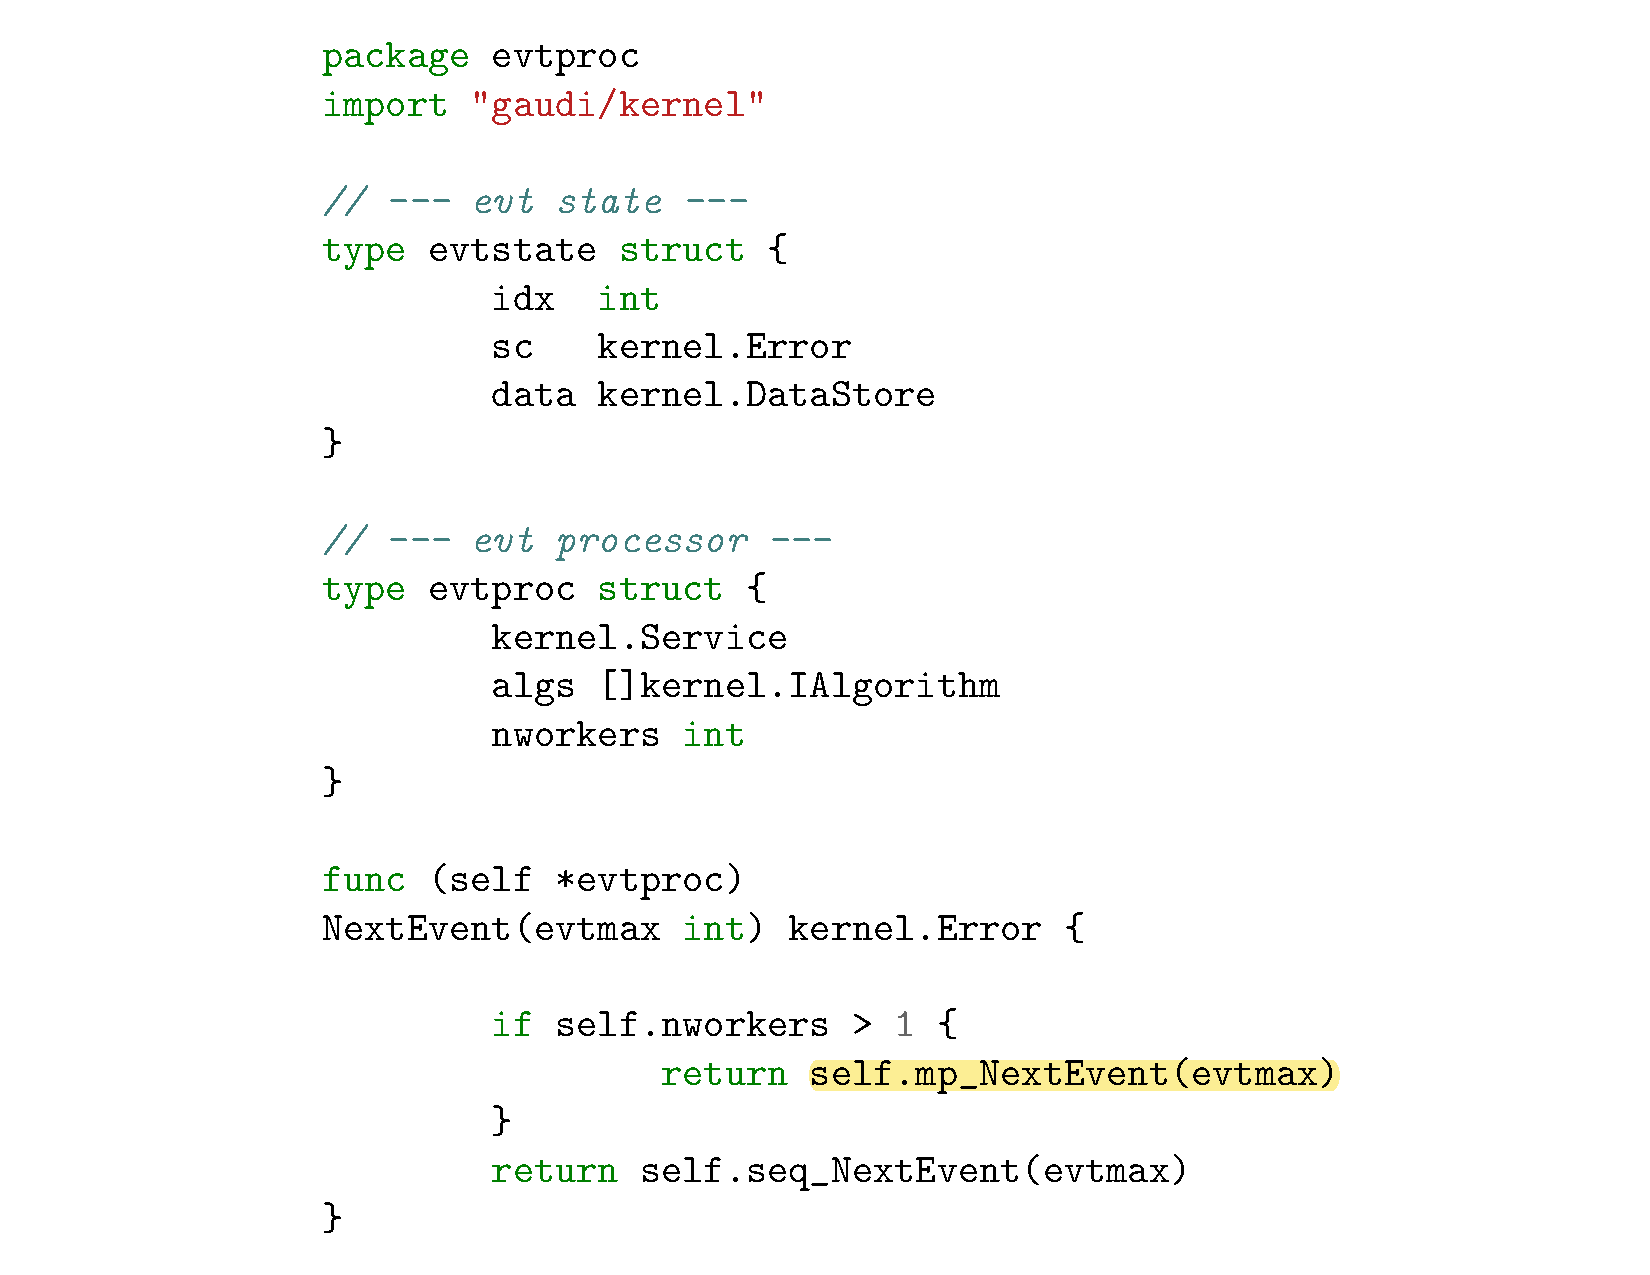
\includegraphics[width=.9\linewidth]{figs/evtproc-mp-next-evt-0-go.pdf}
\end{frame}
\begin{frame}
\frametitle{Go concurrent - IV}
\label{sec-1-13}


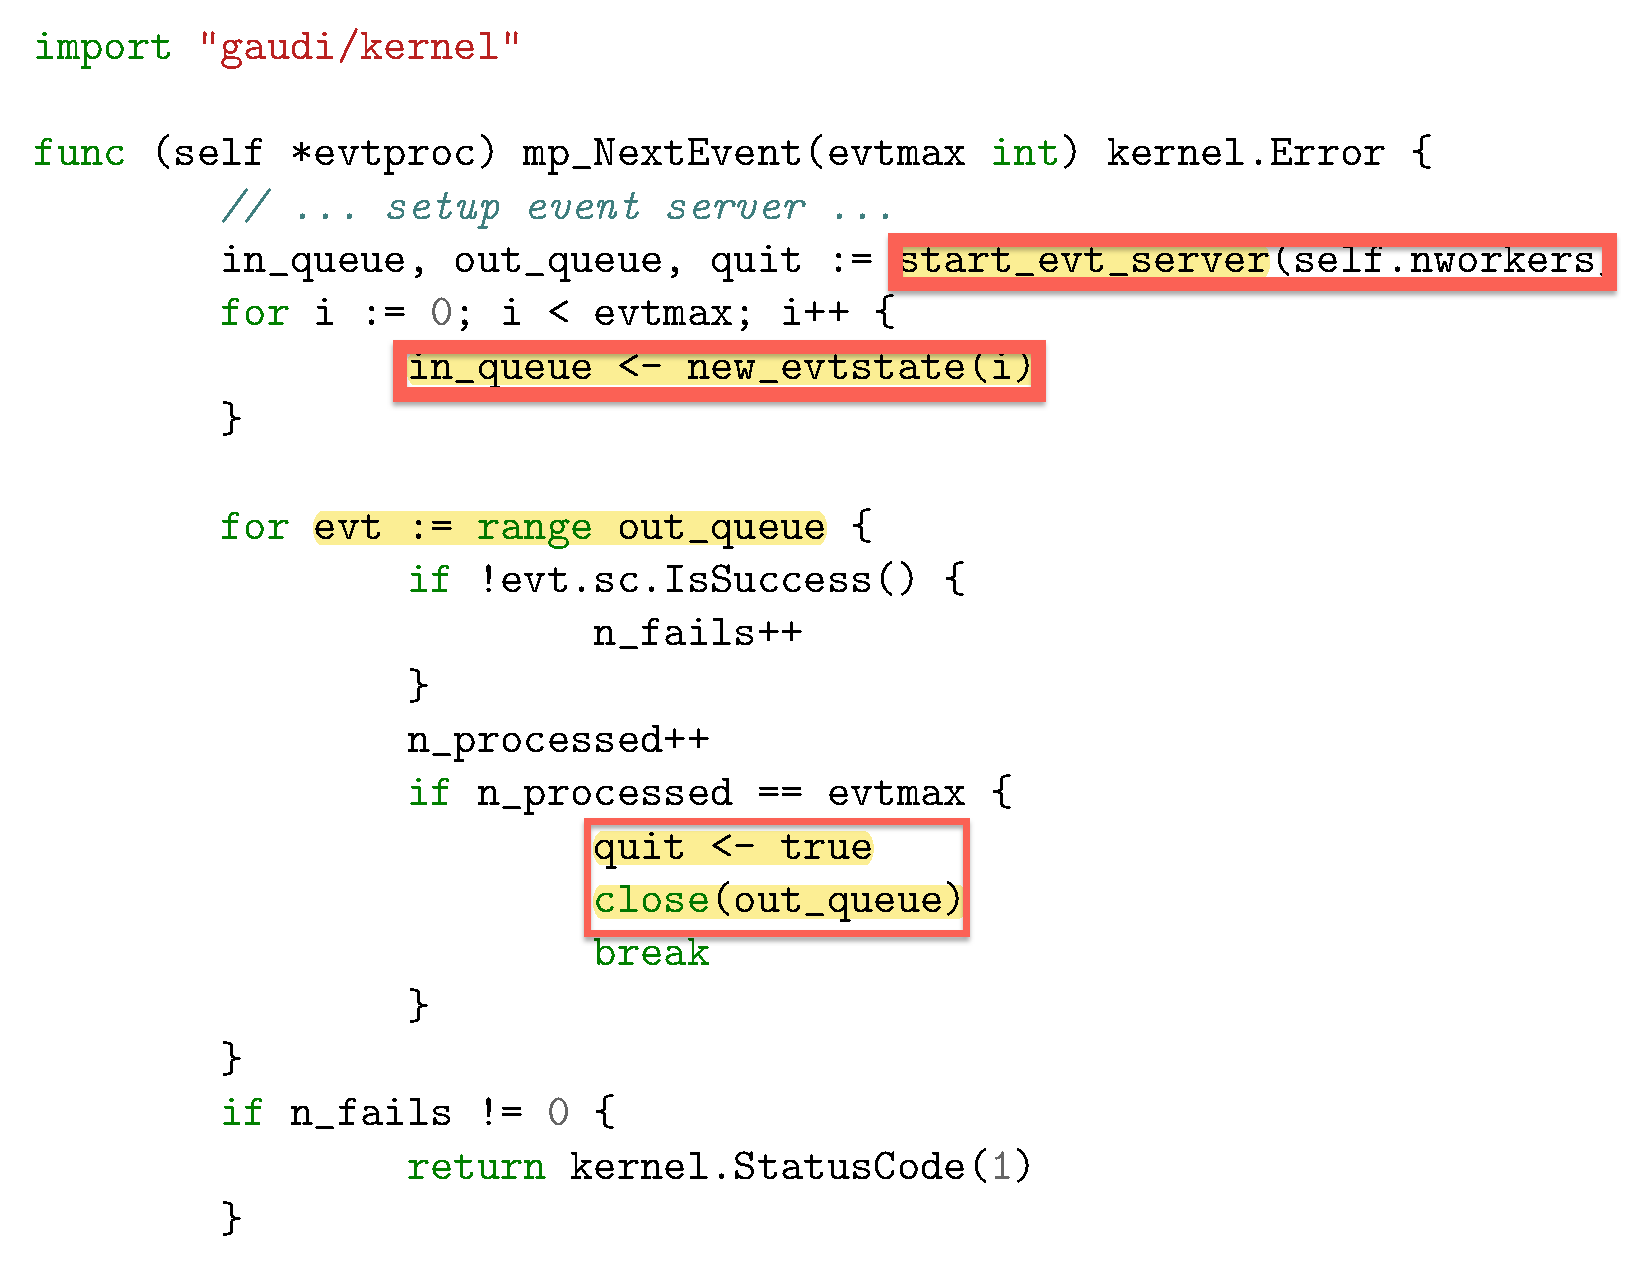
\includegraphics[width=.9\linewidth]{figs/evtproc-mp-next-evt-1-go.pdf}
\end{frame}
\begin{frame}
\frametitle{Go concurrent - V}
\label{sec-1-14}


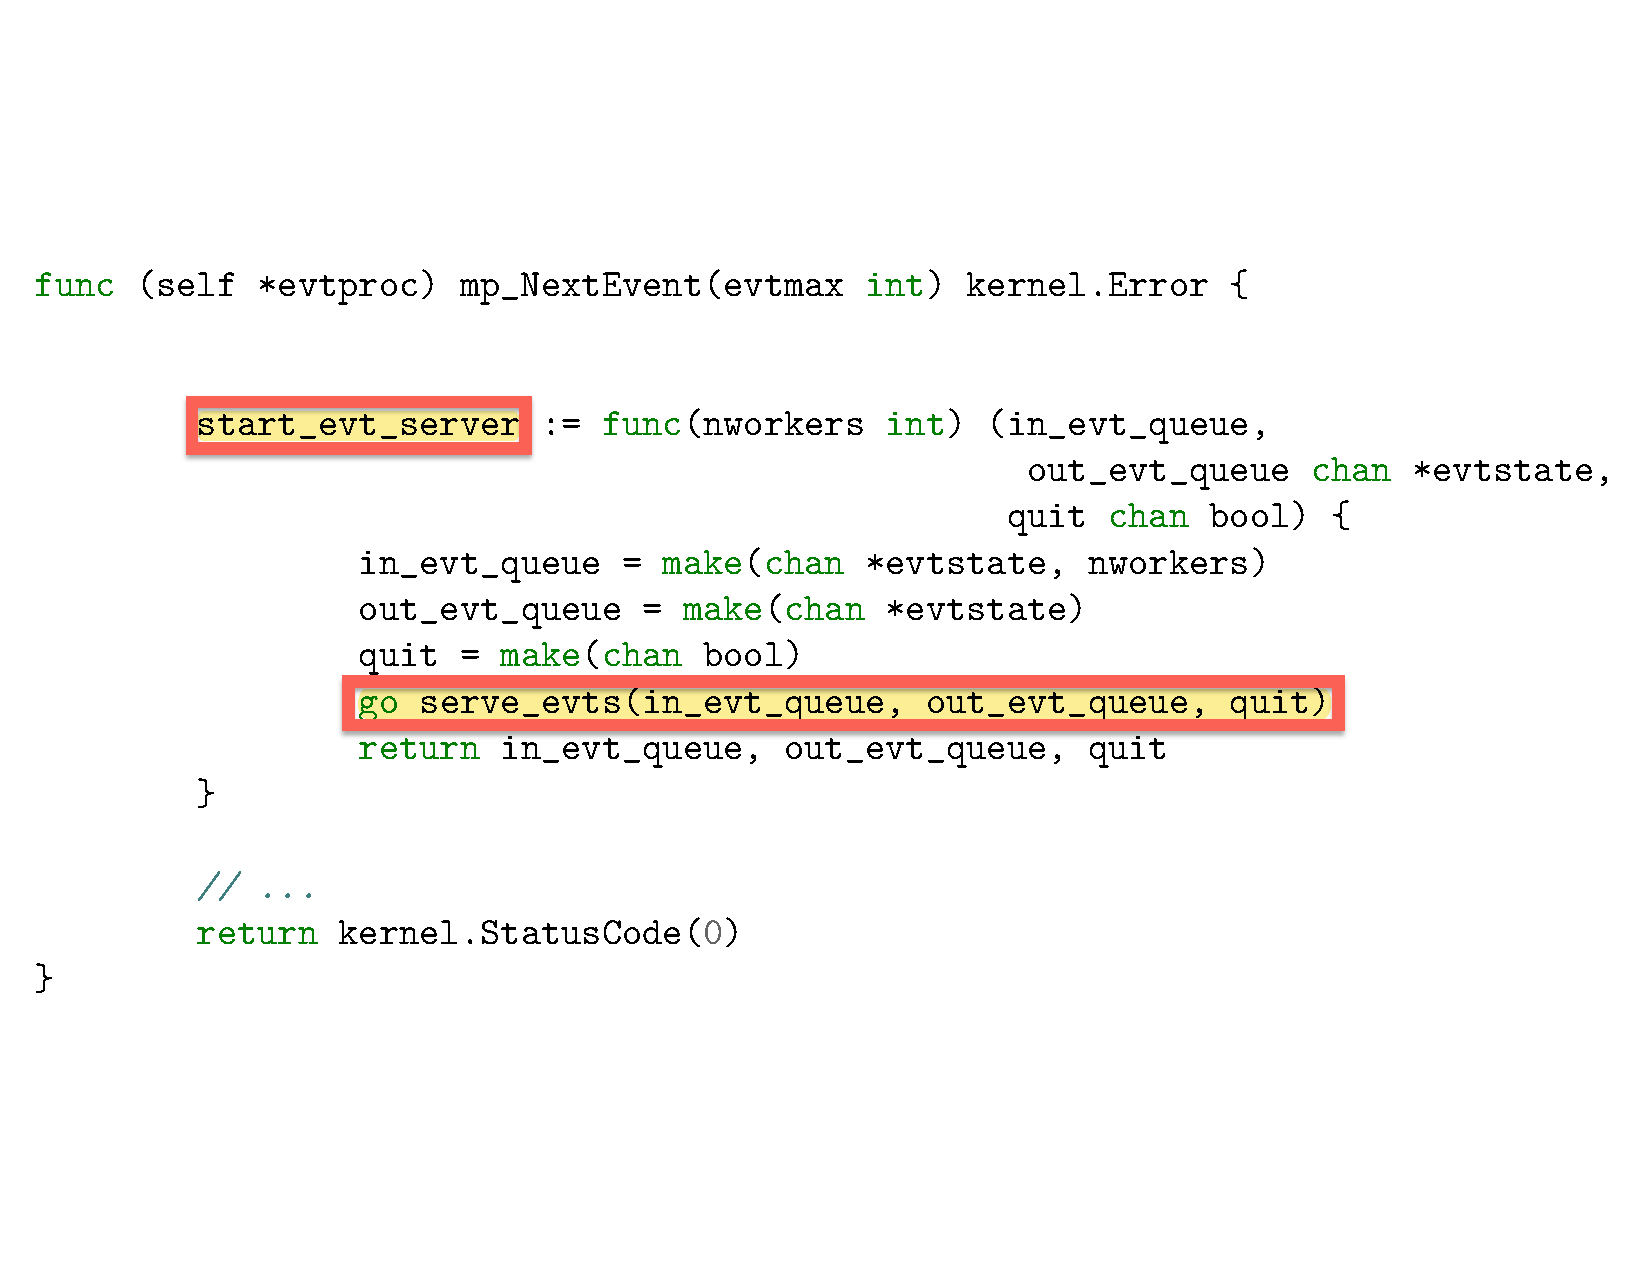
\includegraphics[width=.9\linewidth]{figs/evtproc-mp-next-evt-2-go.pdf}
\end{frame}
\begin{frame}
\frametitle{Go concurrent - VI}
\label{sec-1-15}


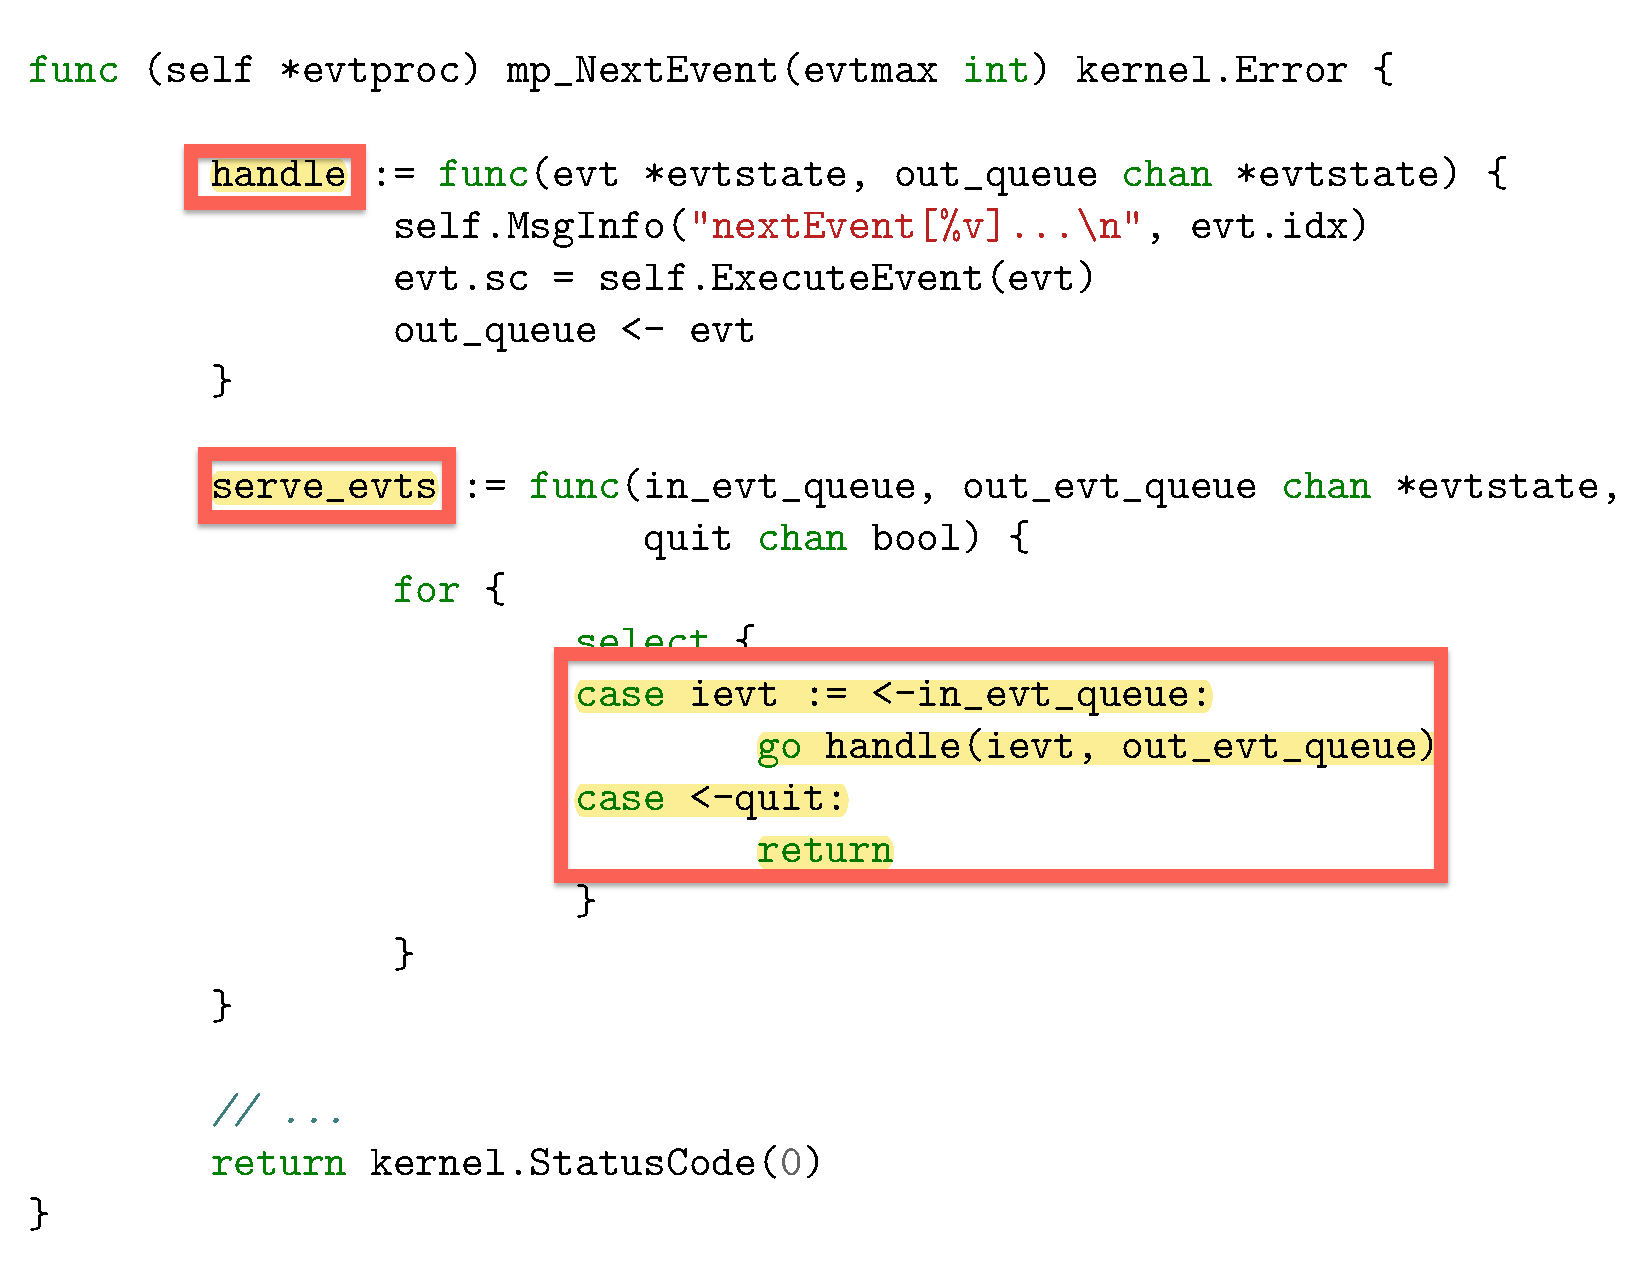
\includegraphics[width=.9\linewidth]{figs/evtproc-mp-next-evt-3-go.pdf}
\end{frame}
\begin{frame}
\frametitle{Go concurrent - VII}
\label{sec-1-16}


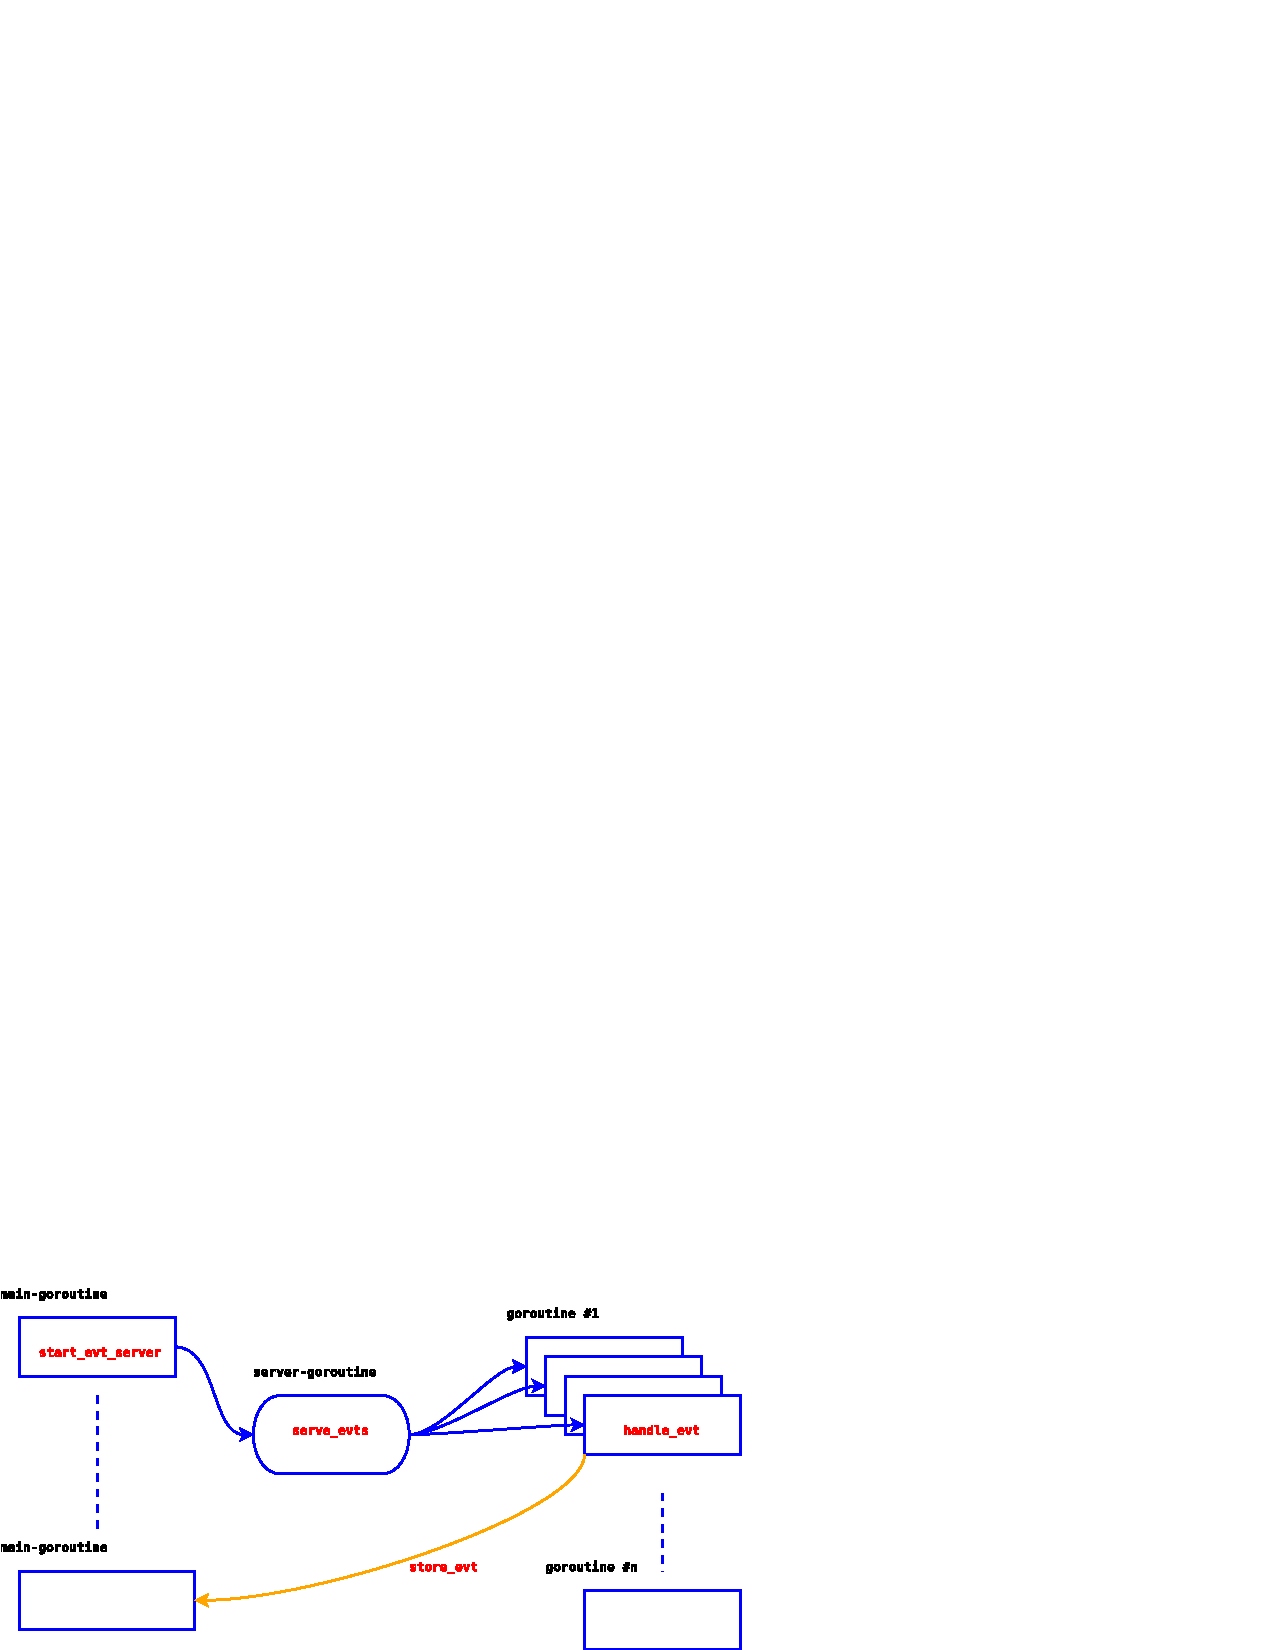
\includegraphics[width=.9\linewidth]{figs/evtproc-diagram.pdf}
\end{frame}
\begin{frame}
\frametitle{Go concurrent with \verb~ng-go-gaudi~}
\label{sec-1-17}


\begin{itemize}
\item very minimal implementation of \verb~Gaudi~ in \verb~Go~:
\begin{itemize}
\item \verb~appmgr~
\item \verb~evtproc~
\item \verb~datastoresvc~
\item \verb~algorithm~, \verb~messages~, \verb~tools~, \verb~services~, \verb~properties~
\item simple \verb~JSON~ output stream
\item simple \verb~go~ bytestream (\verb~gob~) output stream
\item simple test algorithms (\verb~adder, counter, ...~)
\end{itemize}
\end{itemize}
\end{frame}
\begin{frame}
\frametitle{A simple \verb~jobo.py~ example}
\label{sec-1-18}


\begin{itemize}
\item create 500 \verb~adder~ algorithms,  500 \verb~dumper~ algorithms
\item process 10000 events, spawn off 5000 concurrent workers
\end{itemize}

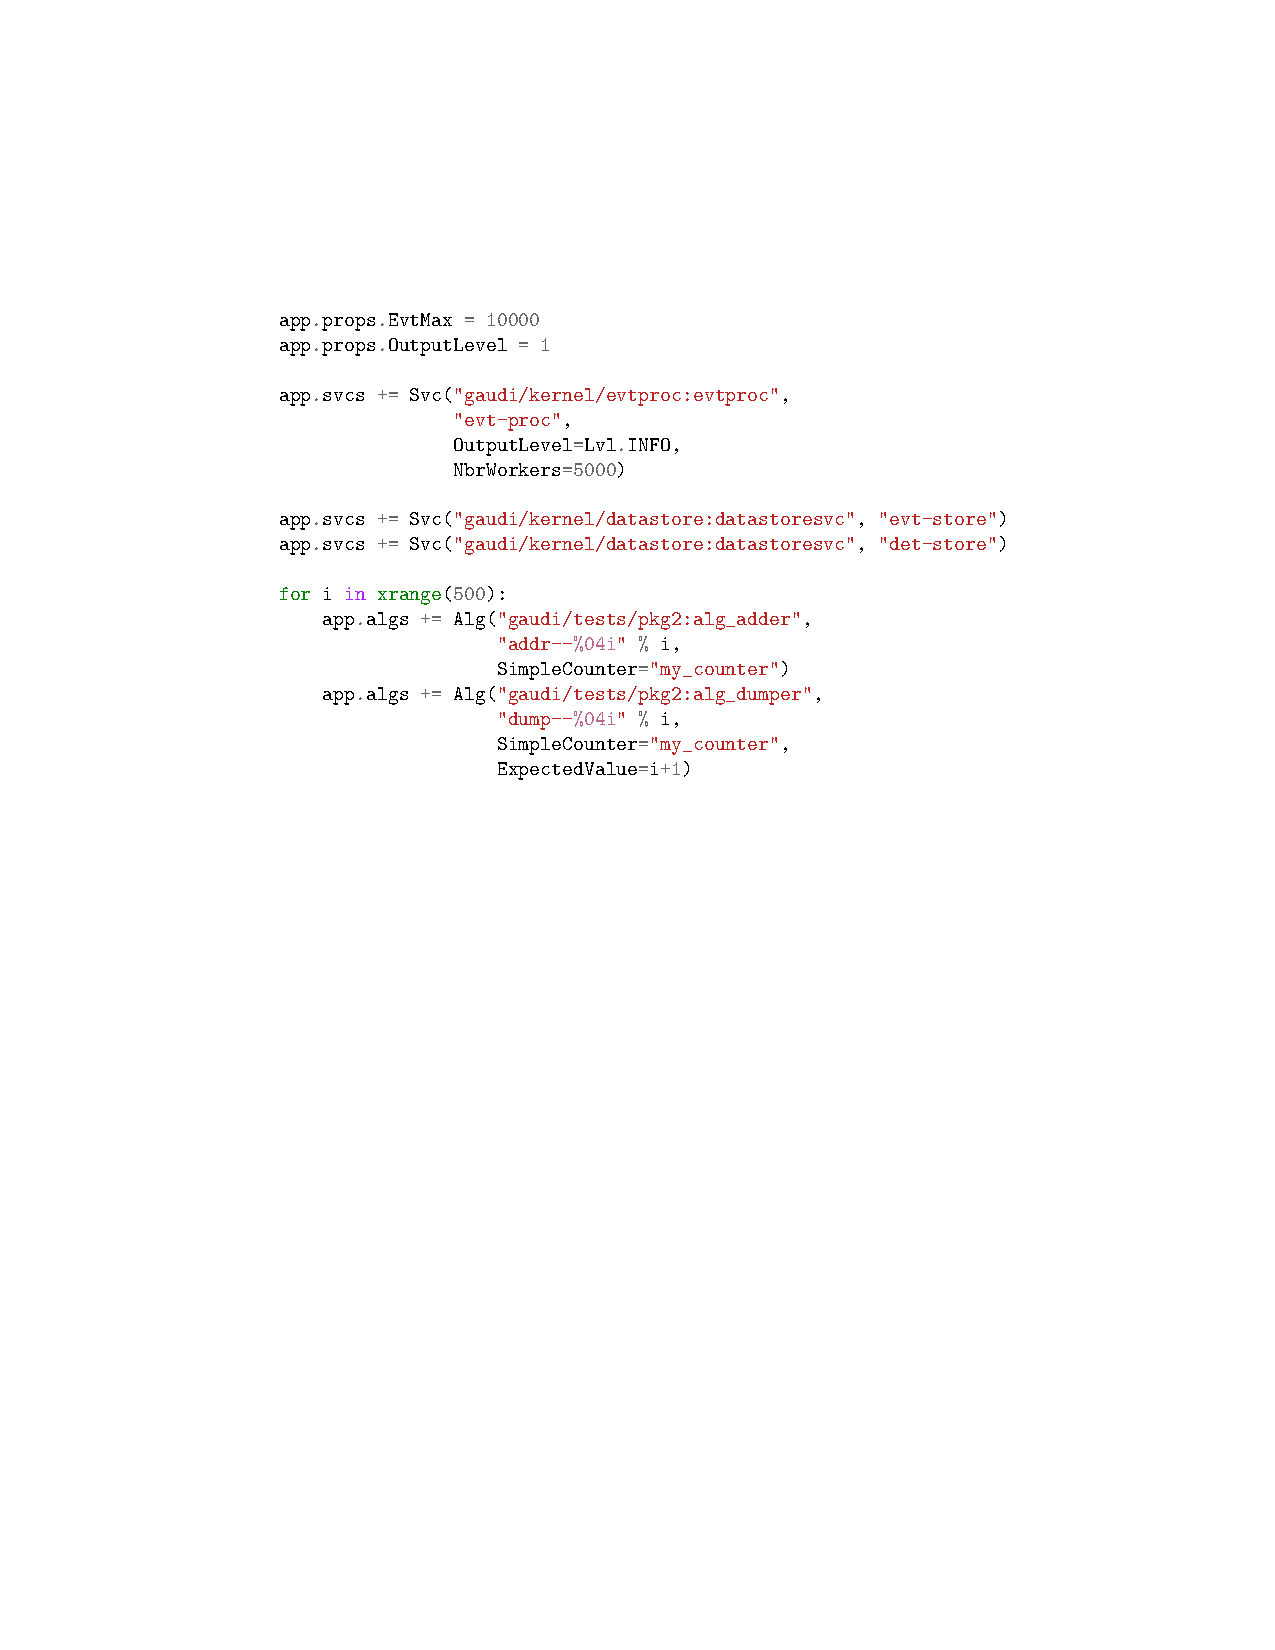
\includegraphics[width=.9\linewidth]{figs/big-jobo.pdf}
\end{frame}
\begin{frame}
\frametitle{Non-elements of \verb~Go~}
\label{sec-1-19}


\begin{itemize}
\item \alert{no} dynamic libraries (frown upon)
\item \alert{no} dynamic loading (yet)
\begin{itemize}
\item but can either rely on separate processes
\begin{itemize}
\item \verb~IPC~ is made easy \emph{via} the \verb~netchan~ package
\end{itemize}
\item or rebuild executables on the fly
\begin{itemize}
\item \alert{compilation} of \verb~Go~ code is \alert{fast}
\item even faster than \verb~FORTRAN~ and/or \verb~C~
\end{itemize}
\end{itemize}
\item \alert{no} templates/generics
\begin{itemize}
\item still open issue
\item looking for the proper \verb~Go~ -friendly design
\end{itemize}
\item \alert{no} operator overloading
\end{itemize}
\end{frame}
\begin{frame}
\frametitle{Go from anywhere to everywhere}
\label{sec-1-20}


\begin{itemize}
\item code compilation and distribution are (\emph{de facto}) standardized
\item put your code on some repository
\begin{itemize}
\item \verb~bitbucket~, \verb~launchpad~, \verb~googlecode~, \verb~github~, \ldots{}
\end{itemize}
\item check out, compile and install in one go with \alert{goinstall}:
\begin{itemize}
\item \verb~goinstall bitbucket.org/binet/igo~
\item no \verb~root~ access required
\item automatically handle \alert{dependencies}
\end{itemize}
\end{itemize}

\vspace

\begin{itemize}
\item \verb~goinstall~ -able packages are listed on the dashboard:
\begin{itemize}
\item \href{http://godashboard.appspot.com}{godashboard.appspot.com}
\end{itemize}
\end{itemize}
\end{frame}
\begin{frame}[fragile]
\frametitle{Go and C/C++}
\label{sec-1-21}


Interfacing with \verb~C~:

\begin{itemize}
\item done with the \verb~CGo~ foreign function interface
\item \verb~#include~ the header file to the \verb~C~ library to be wrapped
\item access the \verb~C~ types and functions under the artificial ``C'' package
\end{itemize}


\begin{minted}[]{go}
package myclib
// #include <stdio.h>
// #include <stdlib.h>
import "C"
import "unsafe"

func foo(s string) {
  c_str := C.CString(s)  // create a C string from a Go one
  C.fputs(c_str, C.stdout)
  C.free(unsafe.Pointer(c_str))
}
\end{minted}
\end{frame}
\begin{frame}
\frametitle{Go and C/C++}
\label{sec-1-22}


Interfacing with \verb~C++~:

\begin{itemize}
\item a bit more involved
\item uses \verb~SWIG~
\begin{itemize}
\item you write the \verb~SWIG~ interface file for the library to be wrapped
\item \verb~SWIG~ will generate the \verb~C~ stub functions
\item which can then be called using the \verb~CGo~ machinery
\item the \verb~Go~ files doing so are automatically generated as well
\end{itemize}
\item handles overloading, multiple inheritance
\item allows to provide a \verb~Go~ implementation for a \verb~C++~ abstract class
\end{itemize}
\begin{alertblock}{Problem}
\label{sec-1-22-1}

    \verb~SWIG~ doesn't understand all of \verb~C++03~
\begin{itemize}
\item \emph{e.g.} can't parse \verb~TObject.h~
\end{itemize}
\end{alertblock}
\end{frame}
\begin{frame}
\frametitle{Go and FORTRAN}
\label{sec-1-23}


Two cases:

\begin{itemize}
\item lucky enough to wrap ``legacy'' \verb~Fortran 03~ code with the \verb~ISO C~
  interface:
\begin{itemize}
\item just use \verb~CGo~
\end{itemize}
\item wrapping legacy \verb~F77~ code:
\begin{itemize}
\item write the \verb~C~ interface code
\item use \verb~CGo~ to call this interface code
\end{itemize}
\item examples:
\begin{itemize}
\item \href{http://bitbucket.org/binet/go-hepevt}{http://bitbucket.org/binet/go-hepevt}
\item \href{http://bitbucket.org/binet/go-herwig}{http://bitbucket.org/binet/go-herwig}
\end{itemize}
\end{itemize}


\begin{itemize}
\item no automatic press-button solution
\begin{itemize}
\item although there is no technical blocker to write such a thing
\item this has been done for \verb~python~ (\emph{e.g.:} \verb~fwrap~)
\end{itemize}
\end{itemize}
\end{frame}
\begin{frame}
\frametitle{Go and ROOT}
\label{sec-1-24}


\begin{itemize}
\item step 1 of evil plan for (\verb~HENP~) world domination:
\begin{itemize}
\item \alert{~Go~ bindings to ~ROOT~}
\end{itemize}
\item \href{http://bitbucket.org/binet/go-croot}{http://bitbucket.org/binet/go-croot}
\begin{itemize}
\item hand written \verb~CGo~ bindings to a hand written library exposing a
    \verb~C~ interface to (a subset of) \verb~ROOT~
\begin{itemize}
\item \verb~TFile~, \verb~TTree/TChain~
\item \verb~Reflex~, \verb~Cint~
\item \verb~TRandom~
\end{itemize}
\item handles automatic conversion of \verb~Go~ structs into their \verb~C~
    counter-part
\item and \emph{vice versa}
\begin{itemize}
\item two-way conversion is done by connecting the \verb~C++~ introspection
      library (\verb~Reflex~) with its \verb~Go~ counter-part (the \verb~reflect~
      package)
\end{itemize}
\end{itemize}
\end{itemize}
\end{frame}
\begin{frame}[fragile]
\frametitle{Go and ROOT}
\label{sec-1-25}


\begin{itemize}
\item running the \verb~ROOT~ \verb~TTree~ example, in \verb~C++~, via the \verb~C API~ and
  through \verb~go-croot~ over 10000000 events:
\end{itemize}

\begin{verbatim}
 29.04s user  1.03s system 86% cpu 34.83 total (C++)
 29.12s user  1.09s system 85% cpu 35.48 total (CRoot)
 44.83s user  1.24s system 87% cpu 54.36 total (go-croot)

$ uname -a
Linux farnsworth 3.0-ARCH #1 SMP PREEMPT 
x86_64 Intel(R) Core(TM)2 Duo 
CPU T9400 @ 2.53GHz GenuineIntel GNU/Linux

\end{verbatim}


additional overhead \emph{w.r.t.} \verb~CRoot~

\begin{itemize}
\item different calling conventions (b/w \verb~C~ and \verb~Go~) need to be handled
\item \emph{Note:} for such loopy-code, using \verb~GCC-Go~ would be better
\end{itemize}
\end{frame}
\begin{frame}
\frametitle{Conclusions}
\label{sec-1-26}


Can \verb~Go~ address the (non-) multicore problems of yesterday ?

\begin{itemize}
\item \alert{yes:}
\begin{itemize}
\item productivity (dev cycle of a scripting language)
\item build scalability (package system)
\item deployment (goinstall)
\item support for ``legacy'' \verb~C/C++/Fortran~ software (cgo+swig)
\end{itemize}
\end{itemize}

\vspace

Can \verb~Go~ address the multicore issues of tomorrow ?

\begin{itemize}
\item \alert{yes:}
\begin{itemize}
\item \alert{easier} to write concurrent code with the builtin abstractions
    (goroutines, channels)
\item \alert{easier} to have efficient concurrent code (stack management)
\item still have to actually write efficient concurrent code, though\ldots{}
\begin{itemize}
\item work partitioning, load balancing, \ldots{}
\end{itemize}
\end{itemize}
\item \textbf{but:} no such thing as a magic wand for multicores/manycores
\end{itemize}
\end{frame}
\begin{frame}
\frametitle{Prospects - what's missing ?}
\label{sec-1-27}


\begin{itemize}
\item better support for \verb~C++~ libraries
\begin{itemize}
\item building on \verb~ROOT~ \verb~C++~ dictionary infrastructure
\begin{itemize}
\item now using \verb~GCC-Xml~ + a modified version of \verb~genreflex~
\item tomorrow using \verb~LLVM/CLang~
\end{itemize}
\item automatically generate the \verb~Go~ bindings
\end{itemize}
\end{itemize}

\vspace

\begin{itemize}
\item bind more \verb~HEP~ libraries ?
\item provide a \verb~Go~ interpreter ?
\begin{itemize}
\item \href{http://bitbucket.org/binet/igo}{bitbucket.org/binet/igo}
\end{itemize}
\end{itemize}
\end{frame}
\begin{frame}
\frametitle{Resources}
\label{sec-1-28}


\begin{itemize}
\item \href{http://golang.org}{golang.org}
\item \href{http://root.cern.ch}{root.cern.ch}
\item \href{http://www.swig.org/}{swig.org}
\item \href{http://godashboard.appspot.com}{godashboard.appspot.com}
\item \href{http://bitbucket.org/binet/go-hepevt}{bitbucket.org/binet/go-hepevt}
\item \href{http://bitbucket.org/binet/go-herwig}{bitbucket.org/binet/go-herwig}
\item \href{http://bitbucket.org/binet/go-croot}{bitbucket.org/binet/go-croot}
\item \href{http://bitbucket.org/binet/ng-go-gaudi}{bitbucket.org/binet/ng-go-gaudi}
\item \href{http://fortrancython.wordpress.com/}{fwrap}
\item \href{http://llvm.org/}{LLVM}
\item \href{http://clang.llvm.org/}{CLang}
\end{itemize}
\end{frame}

\end{document}
